% infrastructure d'un datacenter
Un data center ou centre de donn\'ees est un site physique regroupant des installations informatiques interconnect\'ees (serveurs, r\'eseau informatique, syst\`eme de sauvegarde) et une infrastructure \'energ\'etique ad\'equate (un syst\`eme de distribution \'electrique, un commutateur \'electrique, des r\'eserves d'\'energie, des g\'en\'erateurs d\'edi\'es \`a la sauvegarde de donn\'ees, un syst\`eme de ventilation et de refroidissement).
\newline
% caracteristique du reseau electrique
Le r\'eseau \'electrique est le coeur de data center car il alimente \`a la fois les infrastructures informatique et \'energ\'etique. Il se compose de quatres entit\'es :
\begin{itemize}
\item {\bf Les sources} : 
ces \'equipements sont les points d'entr\'ee de l'\'electricit\'e dans le data center et sont directement rattach\'es au gestionnaire de r\'eseau r\'egional ou national. 
Ils sont de deux types : 
\begin{itemize}
\item Ceux qui alimentent le  r\'eseau en cas de dysfonctionnement du gestionnaire de r\'eseau. Ce sont les accumulateurs, les groupes \'electrog\`enes.
\item Ceux qui transforment l'\'electricit\'e re\c cue du gestionnaire pour des puissances utilisables dans le datacenter. Ce sont les transformateurs basse tension communement appel\'es {\em Transformateur G\'en\'eral Basse Tension (TGBT)}. 
\end{itemize}
G\'en\'eralement, ces deux types d'\'equipements ne fonctionnent pas concomitamment.


\item {\bf Les tableaux} :
aussi appel\'es tableaux de r\'epartition, ce sont des \'equipements passifs dont la fonction est celle de communateur. 
Ils repr\'esentent l'organe central de l'installation dans la mesure o\`u ils regroupent tous les circuits \'electriques et syst\`emes de protection vers les baies de serveurs. 
Une baie est une armoire contenant plusieurs serveurs.
Chaque baie poss\`ede un disjoncteur sur ce tableau afin d'interrompre l'alimentation en cas de danger. 
Les tableaux sont consid\'er\'es comme des \'equipements passifs car l'\'electricit\'e qui traverse ces \'equipements a une perte n\'egligeable.   Ces pertes sont les {\em pertes par Effet Joule}. Un exemple de tableau est pr\'esent\'e dans la figure \`a gauche du tableau \ref{exempleAmoiresTableauxElectriques}. 
%Nous en reparlerons dans la section \ref{pertesEffetsJoules}.

\item {\bf Les baies (ou racks) de serveurs} :
les baies distribuent la puissance n\'ecessaire au fonctionnement de chaque serveur qui lui est rattach\'e. La baie a un r\^ole de multiprise pour tous les serveurs. 
Dans le syst\`eme de supervision \'electrique, les baies sont les consommateurs de l'\'electricit\'e. Elles sont des \'equipements actifs dans le r\'eseau \'electrique.  La figure \`a droite du tableau \ref{exempleAmoiresTableauxElectriques} est un exemple de baie de serveurs. 

\item{\bf Les c\^ables} :
les c\^ables ont pour r\^ole de rattacher les trois entit\'es pr\'ec\'edemment cit\'ees afin de transporter l'\'electricit\'e vers les baies de serveurs. Ils sont caract\'eris\'es par les r\'esistances que nous consid\'erons constantes.
\end{itemize}
% ---- figure exemple amoires ou tableaux electriques et Baie de serveurs 
\begin{table}[htb!] 
	\begin{tabular}{cc}
	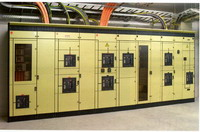
\includegraphics[scale = 1.20]{ReseauFlotsExempleArmoiresTableauxElectriques_okken_PCC.jpg} & 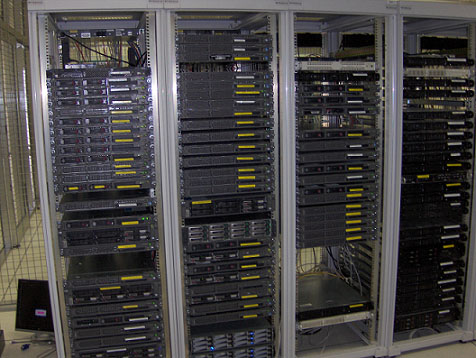
\includegraphics[scale = 0.5]{ReseauFlotsExemple_Baie_serveurs.jpg} \\
	\end{tabular}
	\caption{ Composants \'electriques d'un data center. \`A gauche :  tableaux \'electriques Okken PCC, \`a Droite : baie de serveurs (source: news.pixelistes.com). }
\label{exempleAmoiresTableauxElectriques}
\end{table}

% ---- figure exemple amoires et tableaux electriques


